% ---
% Inicia os anexos
% ---
\begin{anexosenv}

% Imprime uma página indicando o início dos anexos
\partanexos

% ---
\chapter{Conversão \textit{Strokes}-\textit{Flashes}: Teste de Sensibilidade de $\epsilon_{spc}$}
\label{anexo_conversao}

As \autoref{flash_stats_1km}, \autoref{flash_stats_2.5km}, \autoref{flash_stats_5km}, \autoref{flash_stats_10km} mostram 


\begin{figure}[hp]
	\begin{center}
		\caption{Histogramas de tempo entre strokes e entre \textit{flashes} (a), número de \textit{strokes} por \textit{flash} (b) e distância latitude e longitudinal entre \textit{strokes} em um \textit{flash} (c) para diferentes valores de $\epsilon_{\text{spc}}$} 
		\label{flash_stats_mult1}
		%		\setcaptionmargin{1cm}
		\subfloat[$\epsilon_{\text{spc}}=1\:km$]{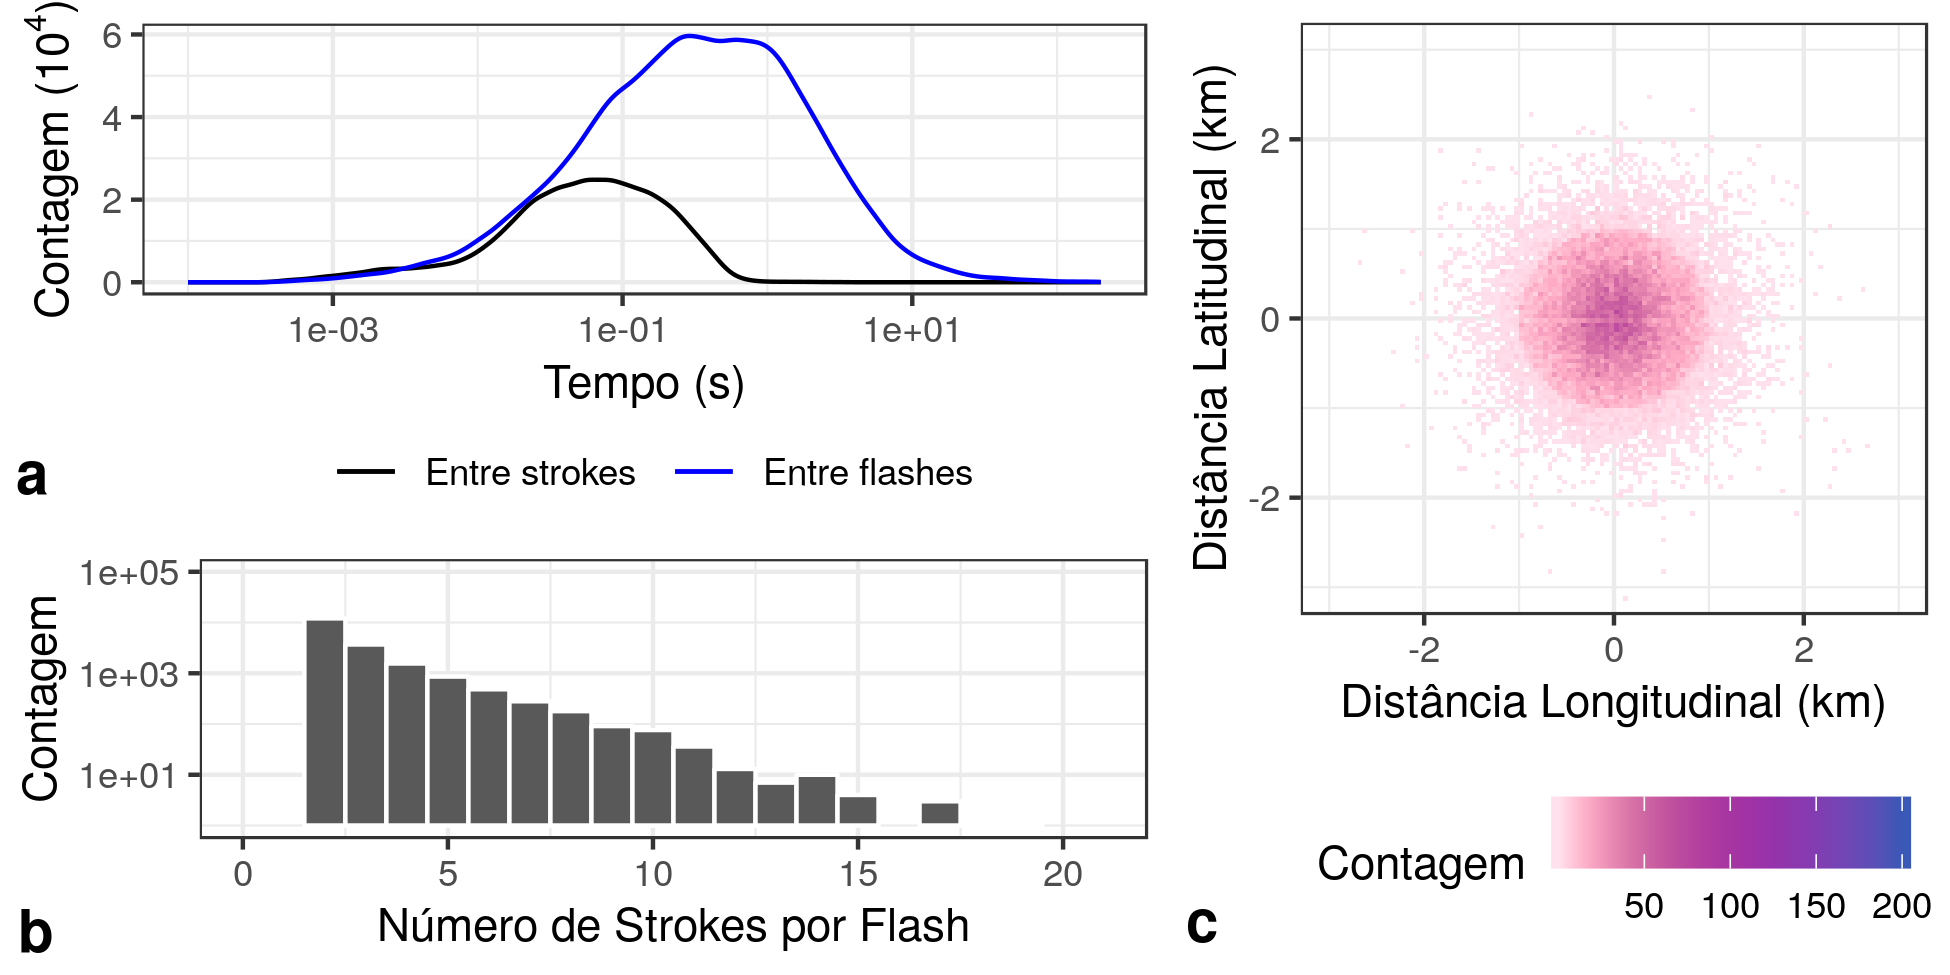
\includegraphics[width=\columnwidth]{../Lightning_Processing/figures/brasildat_flash_stats_1km_ptbr.png}
			\label{flash_stats_1km}} \\
		\subfloat[$\epsilon_{\text{spc}}=2,5\:km$]{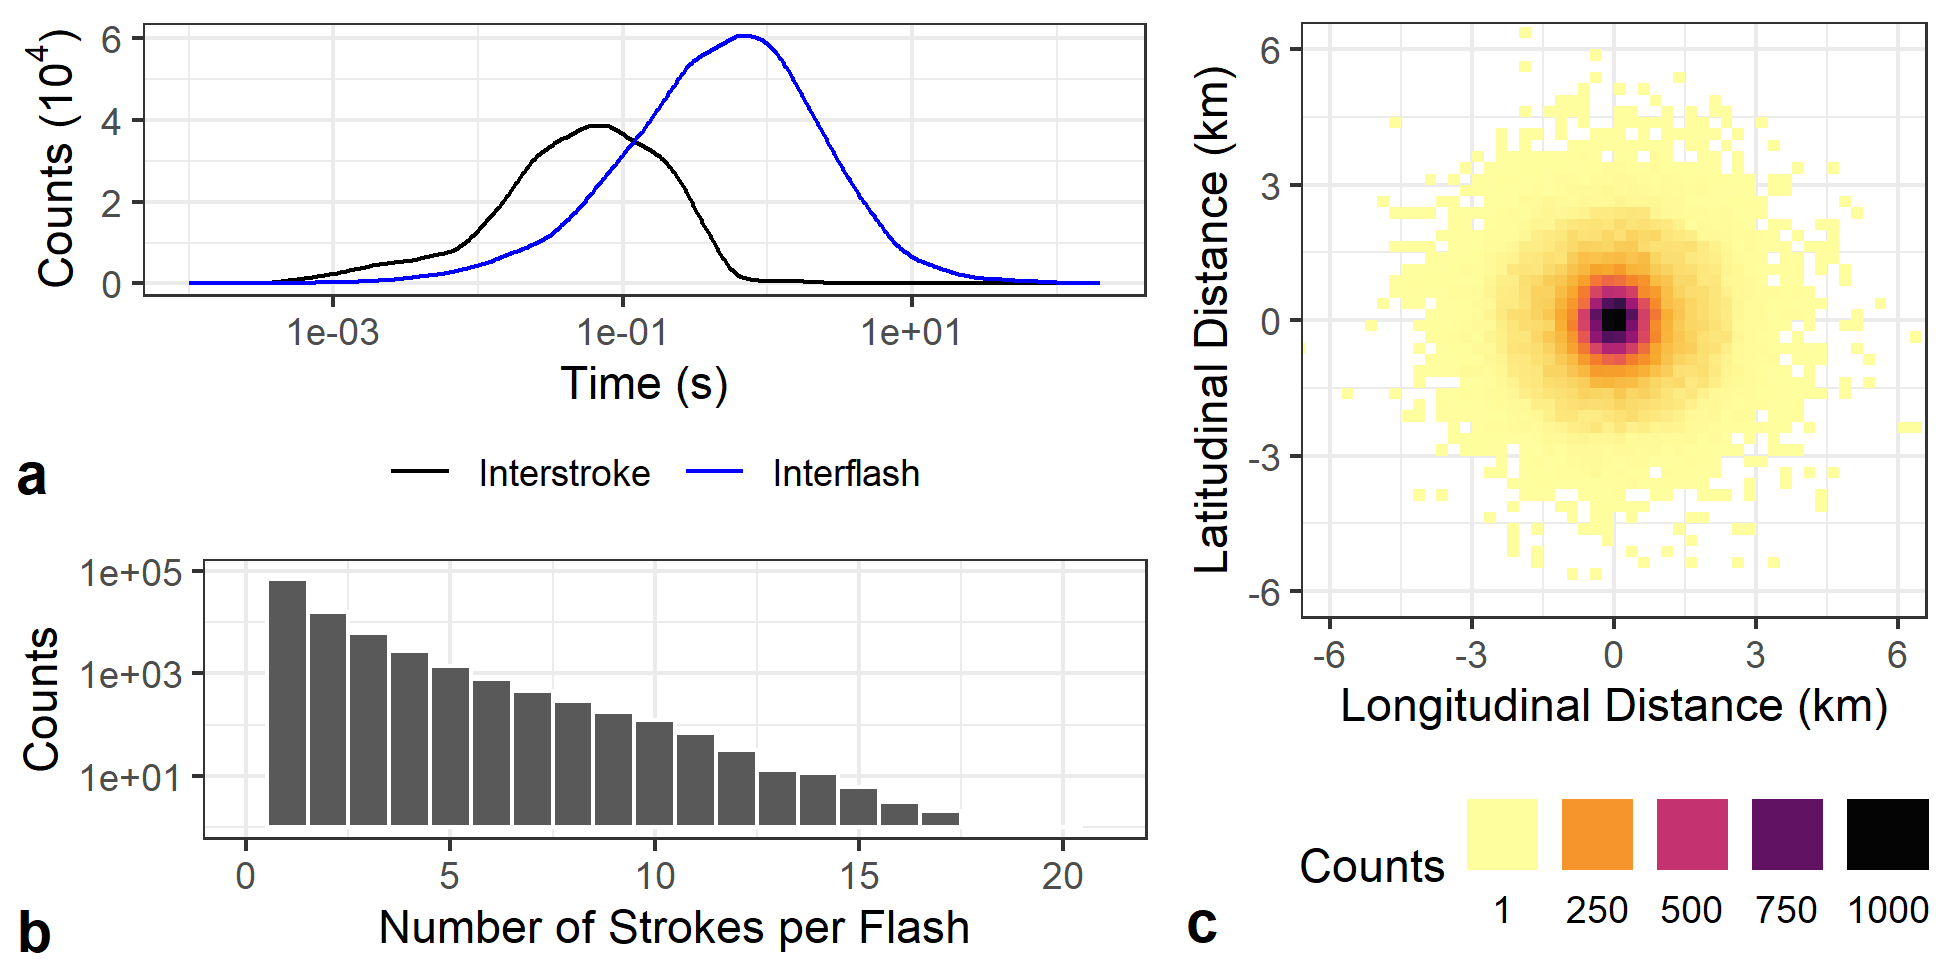
\includegraphics[width=\columnwidth]{../Lightning_Processing/figures/brasildat_flash_stats_ptbr.png}
			\label{flash_stats_2.5km}} \\
		\legend{Fonte: Produzido pela autora.}
	\end{center}
\end{figure}

\begin{figure}[hp]
	\begin{center}
		\caption{Histogramas de tempo entre strokes e entre \textit{flashes} (a), número de \textit{strokes} por \textit{flash} (b) e distância latitude e longitudinal entre \textit{strokes} em um \textit{flash} (c) para diferentes valores de $\epsilon_{\text{spc}}$ - continuação} 
		\label{flash_stats_mult2}
		%		\setcaptionmargin{1cm}
		\subfloat[$\epsilon_{\text{spc}}=5\:km$]{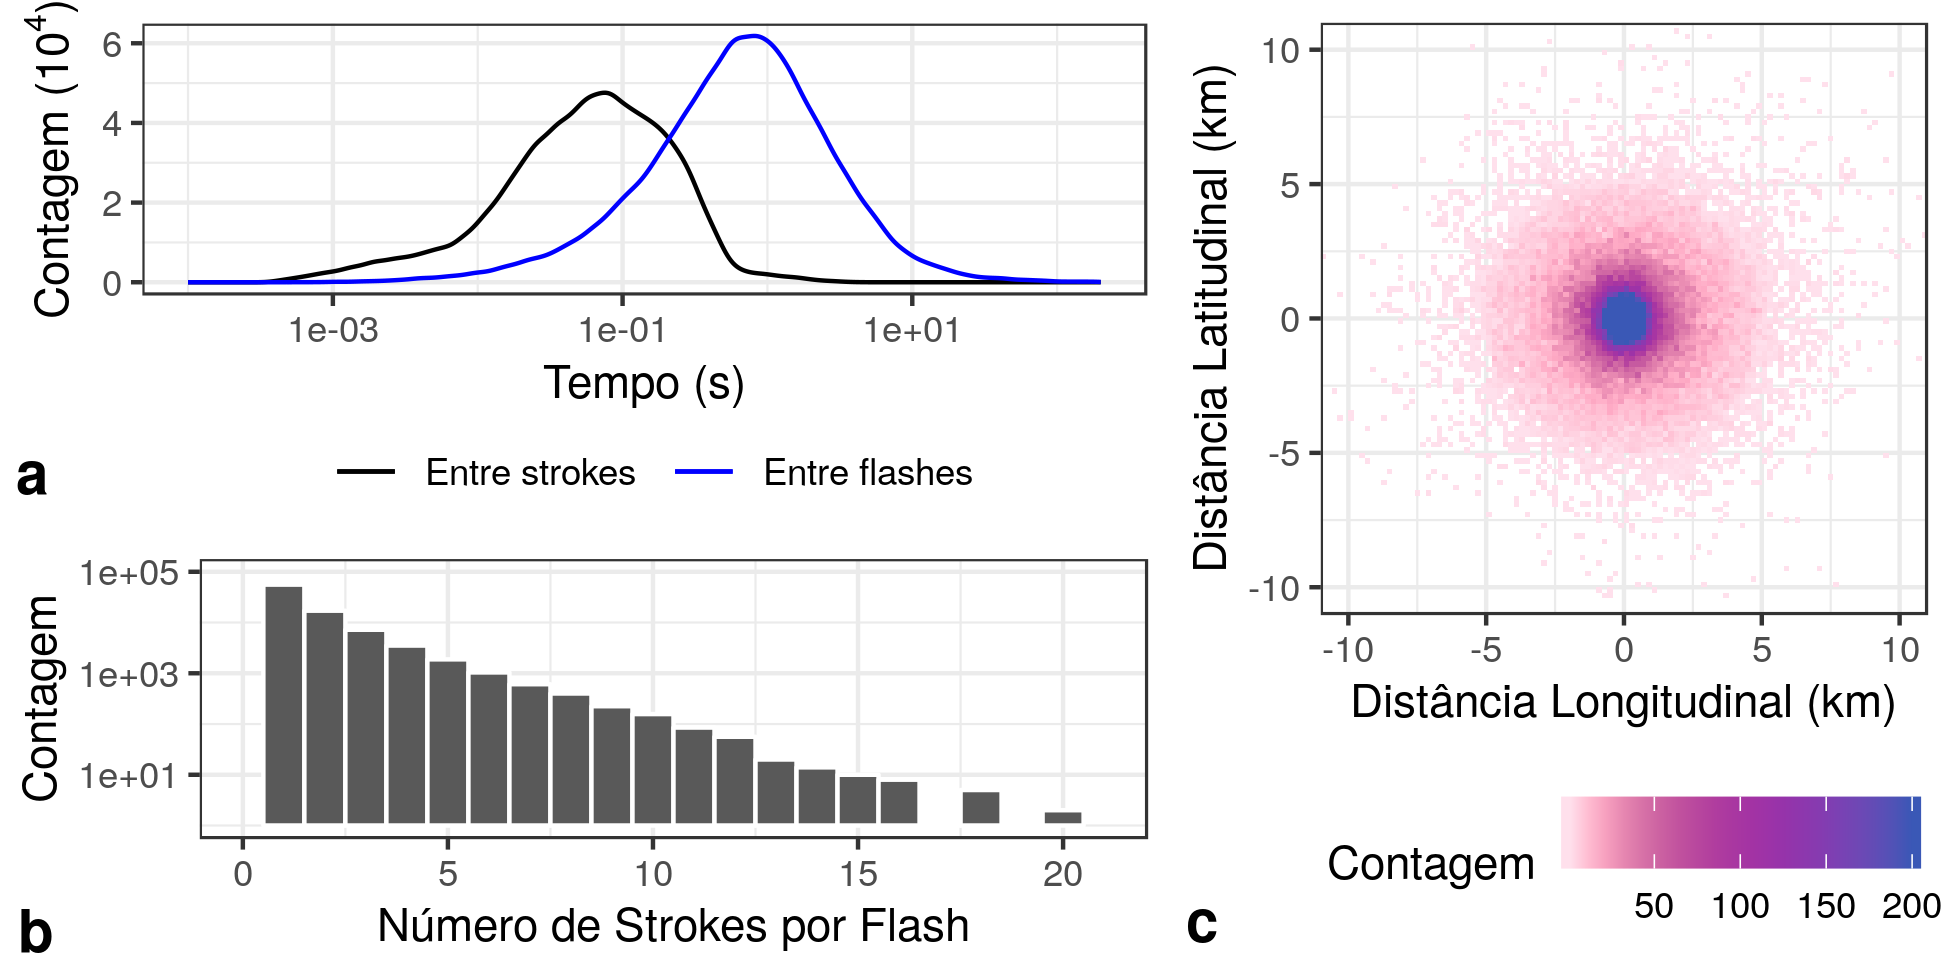
\includegraphics[width=\columnwidth]{../Lightning_Processing/figures/brasildat_flash_stats_5km_ptbr.png}
			\label{flash_stats_5km}} \\
		\subfloat[$\epsilon_{\text{spc}}=10\:km$]{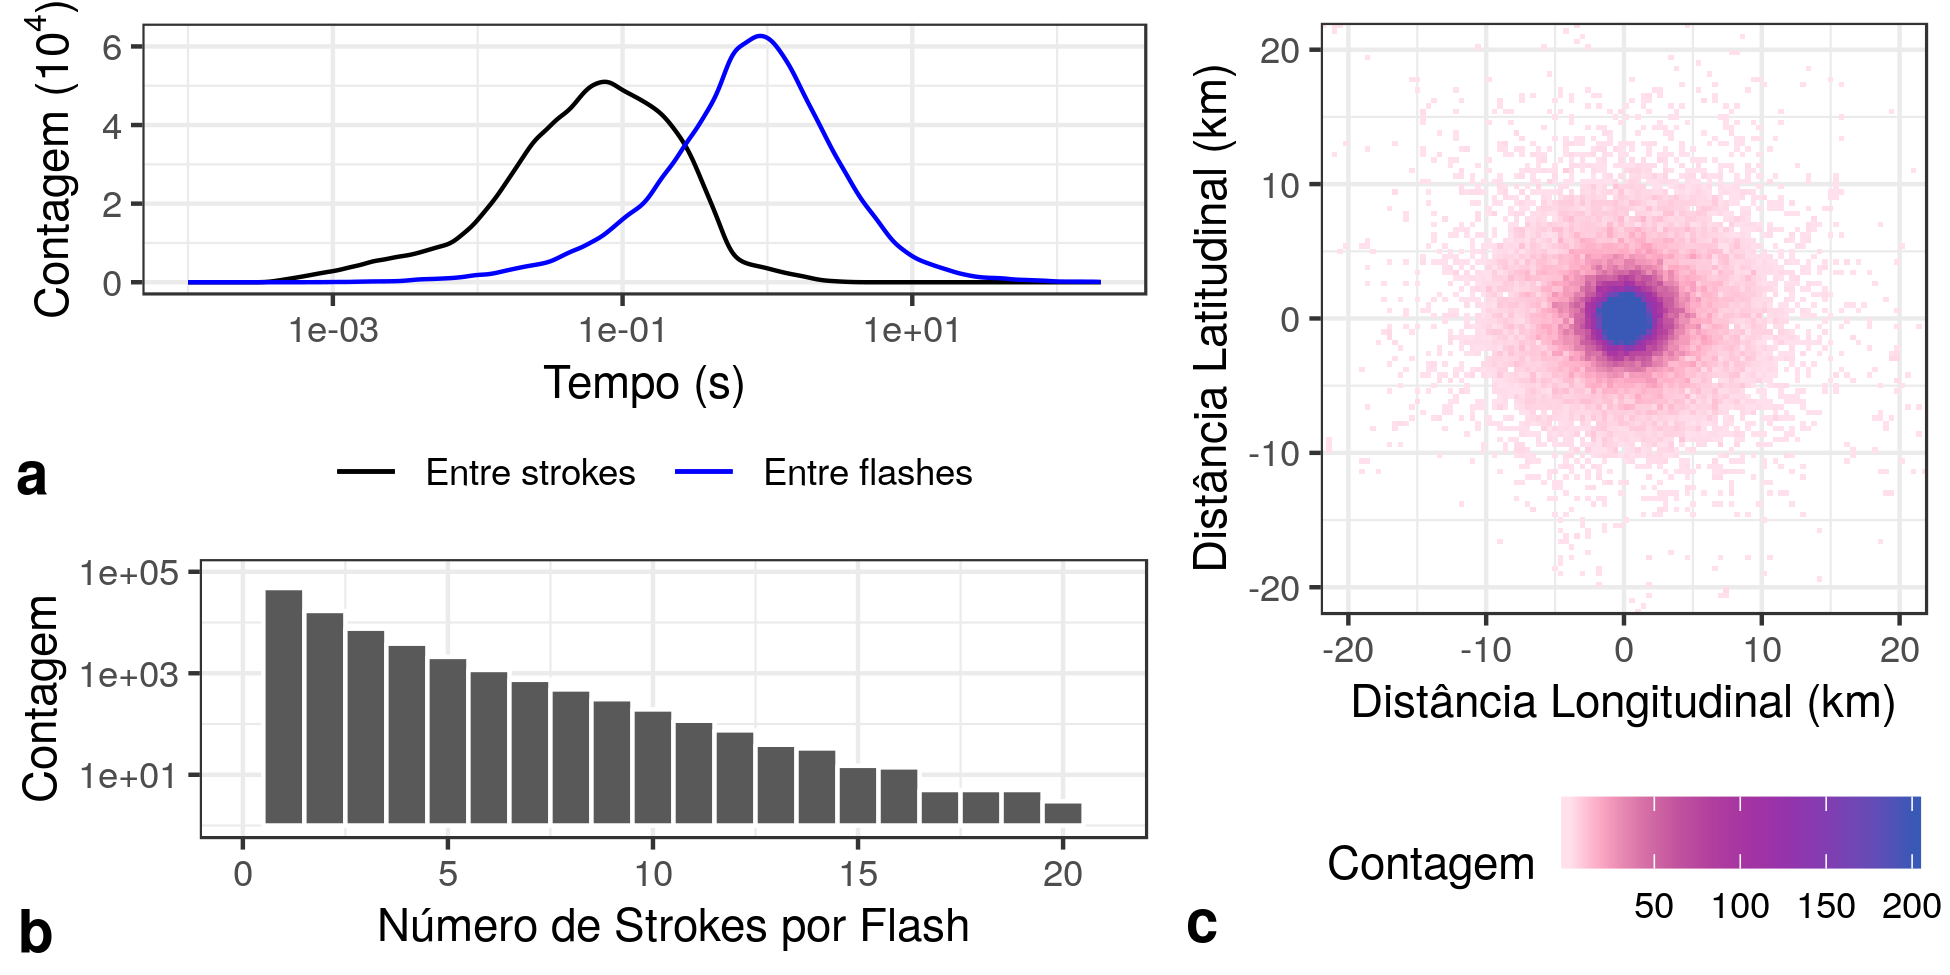
\includegraphics[width=\columnwidth]{../Lightning_Processing/figures/brasildat_flash_stats_10km_ptbr.png}
			\label{flash_stats_10km}} \\
		\legend{Fonte: Produzido pela autora.}
	\end{center}
\end{figure}

\end{anexosenv}
